% ============================================================
% 讲义 — 人教版七年级下册 第9章 不等式与不等式组
% 编译命令：xelatex -interaction=nonstopmode 第9章_不等式与不等式组.tex
% ============================================================
\documentclass[12pt, a4paper]{ctexart}
\usepackage[margin=2.2cm]{geometry}
\usepackage{amsmath, amssymb}
\usepackage{enumitem}
\usepackage{tcolorbox}
\usepackage{booktabs}
\usepackage{array}
\usepackage{fancyhdr}
\usepackage{xcolor}
\usepackage{tikz}
\usepackage{hyperref}
\usepackage{graphicx}
\usepackage{multirow}
\usepackage{pgfplots}
\pgfplotsset{compat=1.18}

% 颜色定义
\definecolor{mainblue}{RGB}{41, 98, 168}
\definecolor{lightblue}{RGB}{230, 240, 255}
\definecolor{tipgreen}{RGB}{34, 139, 87}
\definecolor{lightgreen}{RGB}{235, 250, 240}
\definecolor{warnred}{RGB}{200, 50, 50}
\definecolor{lightred}{RGB}{255, 240, 240}
\definecolor{examorange}{RGB}{210, 120, 20}
\definecolor{lightorange}{RGB}{255, 248, 235}
\definecolor{apppurple}{RGB}{120, 60, 170}
\definecolor{lightpurple}{RGB}{245, 238, 255}

% 页眉页脚
\pagestyle{fancy}
\fancyhf{}
\fancyhead[L]{\small\textcolor{mainblue}{\textbf{人教版七年级下册 · 第9章 不等式与不等式组}}}
\fancyhead[R]{\small\textcolor{mainblue}{家教讲义}}
\fancyfoot[C]{\small —\ \thepage\ —}
\renewcommand{\headrulewidth}{0.6pt}
\renewcommand{\headrule}{\hbox to\headwidth{\color{mainblue}\leaders\hrule height \headrulewidth\hfill}}
\renewcommand{\footrulewidth}{0pt}

% tcolorbox 样式
\newtcolorbox{knowledgebox}[1][]{%
  colback=lightblue, colframe=mainblue,
  fonttitle=\bfseries\large, title=#1,
  arc=3mm, boxrule=0.8pt,
  left=8pt, right=8pt, top=6pt, bottom=6pt
}

\newtcolorbox{tipbox}[1][]{%
  colback=lightgreen, colframe=tipgreen,
  fonttitle=\bfseries, title=#1,
  arc=2mm, boxrule=0.6pt,
  left=6pt, right=6pt, top=4pt, bottom=4pt
}

\newtcolorbox{warnbox}[1][]{%
  colback=lightred, colframe=warnred,
  fonttitle=\bfseries, title=#1,
  arc=2mm, boxrule=0.6pt,
  left=6pt, right=6pt, top=4pt, bottom=4pt
}

\newtcolorbox{examplebox}[1][]{%
  colback=lightorange, colframe=examorange,
  fonttitle=\bfseries, title=#1,
  arc=3mm, boxrule=0.8pt,
  left=8pt, right=8pt, top=6pt, bottom=6pt
}

\newtcolorbox{appbox}[1][]{%
  colback=lightpurple, colframe=apppurple,
  fonttitle=\bfseries, title=#1,
  arc=3mm, boxrule=0.8pt,
  left=8pt, right=8pt, top=6pt, bottom=6pt
}

\setCJKmainfont{Hiragino Sans GB}
\setCJKsansfont{Heiti SC}

\begin{document}

% ============ 标题页 ============
\begin{center}
{\Huge\bfseries\textcolor{mainblue}{第9章\quad 不等式与不等式组}}\\[12pt]
{\Large\textcolor{gray}{讲\quad 义}}\\[8pt]
\rule{0.6\textwidth}{1pt}\\[8pt]
{\normalsize 适用：人教版\quad 七年级下册\quad |\quad 课时：4课时}
\end{center}
\vspace{10pt}

% ============ 第一部分：知识点讲解 ============
\section*{\textcolor{mainblue}{一、知识点讲解}}

\subsection*{9.1\quad 不等式的概念}

\begin{knowledgebox}[9.1.1 不等式]
用不等号（$>$、$<$、$\geqslant$、$\leqslant$、$\neq$）连接的式子叫做\textbf{不等式}。

例如：$3 > 2$，$x + 1 < 5$，$2a \geqslant 0$ 都是不等式。

\vspace{4pt}
\textbf{常见不等号含义：}
\begin{itemize}[leftmargin=2em]
  \item $>$：大于；\quad $<$：小于
  \item $\geqslant$：大于或等于（不小于）；\quad $\leqslant$：小于或等于（不大于）
  \item $\neq$：不等于
\end{itemize}
\end{knowledgebox}

\subsection*{9.2\quad 不等式的基本性质}

\begin{knowledgebox}[9.2.1 不等式的基本性质1]
\textbf{性质1：}不等式两边都加上（或减去）同一个数或同一个整式，不等号的方向\textbf{不变}。

即：若 $a > b$，则 $a + c > b + c$，$a - c > b - c$。
\end{knowledgebox}

\begin{knowledgebox}[9.2.2 不等式的基本性质2]
\textbf{性质2：}不等式两边都乘以（或除以）同一个\textbf{正数}，不等号的方向\textbf{不变}。

即：若 $a > b$，$c > 0$，则 $ac > bc$，$\dfrac{a}{c} > \dfrac{b}{c}$。
\end{knowledgebox}

\begin{knowledgebox}[9.2.3 不等式的基本性质3]
\textbf{性质3：}不等式两边都乘以（或除以）同一个\textbf{负数}，不等号的方向\textbf{改变}。

即：若 $a > b$，$c < 0$，则 $ac < bc$，$\dfrac{a}{c} < \dfrac{b}{c}$。
\end{knowledgebox}

\begin{warnbox}[易错提醒：性质3]
性质3是最容易出错的地方！乘以或除以负数时，不等号必须\textbf{反向}。

\textbf{典型错误：}已知 $-2x > 6$，两边除以 $-2$，得 $x > 3$。

\textbf{正确做法：}两边除以 $-2$，不等号反向，得 $x < -3$。
\end{warnbox}

\begin{tipbox}[不等式性质与等式性质的对比]
\renewcommand{\arraystretch}{1.3}
\begin{center}
\begin{tabular}{|c|c|c|}
\hline
 & \textbf{等式性质} & \textbf{不等式性质} \\
\hline
两边加减同数 & 仍相等 & 不等号方向不变 \\
\hline
两边乘除同正数 & 仍相等 & 不等号方向不变 \\
\hline
两边乘除同负数 & 仍相等 & \textbf{不等号方向改变！} \\
\hline
\end{tabular}
\end{center}
\end{tipbox}

\subsection*{9.3\quad 一元一次不等式及其解法}

\begin{knowledgebox}[9.3.1 一元一次不等式]
只含有\textbf{一个}未知数，未知数的次数是\textbf{1}，且不等号两边都是整式的不等式，叫做\textbf{一元一次不等式}。

例如：$2x - 1 > 3$，$\dfrac{x}{2} + 5 \leqslant 10$。
\end{knowledgebox}

\begin{knowledgebox}[9.3.2 一元一次不等式的解法步骤]
解一元一次不等式的步骤与解一元一次方程类似：
\begin{enumerate}[leftmargin=2em]
  \item \textbf{去分母}：不等式两边同乘各分母的最小公倍数（注意不等号方向！）
  \item \textbf{去括号}：利用乘法分配律展开
  \item \textbf{移项}：把含未知数的项移到一边，常数项移到另一边（变号）
  \item \textbf{合并同类项}：化为 $ax > b$ 或 $ax < b$ 的形式
  \item \textbf{系数化为1}：两边同除以 $a$。若 $a < 0$，不等号要\textbf{反向}！
\end{enumerate}
\end{knowledgebox}

\begin{tipbox}[解集的概念]
一个不等式的\textbf{所有解}组成的集合，叫做这个不等式的\textbf{解集}。

例如：$x > 3$ 的解集是所有大于3的实数。
\end{tipbox}

\subsection*{9.4\quad 在数轴上表示不等式的解集}

\begin{knowledgebox}[9.4.1 数轴表示法]
在数轴上表示不等式的解集时：
\begin{itemize}[leftmargin=2em]
  \item 向\textbf{右}画表示大于，向\textbf{左}画表示小于
  \item 端点处画\textbf{空心圆圈}（$\circ$）：表示\textbf{不包含}该数（$>$、$<$）
  \item 端点处画\textbf{实心圆圈}（$\bullet$）：表示\textbf{包含}该数（$\geqslant$、$\leqslant$）
\end{itemize}

\textbf{示例：}在数轴上表示 $x \geqslant -2$：

\begin{center}
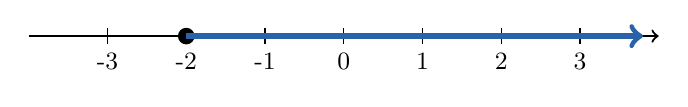
\begin{tikzpicture}
  \draw[->, thick] (-4, 0) -- (4, 0);
  \foreach \x in {-3,-2,-1,0,1,2,3}
    \draw (\x, 0.1) -- (\x, -0.1) node[below] {\small \x};
  \fill (-2, 0) circle (3pt);
  \draw[thick, mainblue, line width=2pt] (-2, 0) -- (3.5, 0);
  \draw[->, thick, mainblue, line width=2pt] (3.5, 0) -- (3.8, 0);
\end{tikzpicture}
\end{center}
\end{knowledgebox}

\subsection*{9.5\quad 一元一次不等式组}

\begin{knowledgebox}[9.5.1 不等式组及其解集]
把两个（或两个以上）一元一次不等式合在一起，就组成一个\textbf{一元一次不等式组}。

不等式组的解集是各个不等式解集的\textbf{公共部分}（交集）。
\end{knowledgebox}

\begin{knowledgebox}[9.5.2 不等式组解集的四种情况]
设 $a < b$，一元一次不等式组的解集有以下四种情况：

\renewcommand{\arraystretch}{1.5}
\begin{center}
\begin{tabular}{|c|c|c|}
\hline
\textbf{类型} & \textbf{不等式组} & \textbf{解集（口诀）} \\
\hline
同大取大 & $\begin{cases} x > a \\ x > b \end{cases}$ & $x > b$ \\
\hline
同小取小 & $\begin{cases} x < a \\ x < b \end{cases}$ & $x < a$ \\
\hline
大小小大取中间 & $\begin{cases} x > a \\ x < b \end{cases}$ & $a < x < b$ \\
\hline
大大小小无解 & $\begin{cases} x < a \\ x > b \end{cases}$ & 无解 \\
\hline
\end{tabular}
\end{center}
\end{knowledgebox}

\begin{tipbox}[记忆口诀]
\textbf{同大取大，同小取小，大小小大取中间，大大小小无解。}

用数轴辅助理解最直观：在数轴上分别画出每个不等式的解集，重叠部分就是不等式组的解集。
\end{tipbox}

\begin{warnbox}[易错提醒]
\begin{itemize}[leftmargin=2em]
  \item 解不等式组时，\textbf{每个}不等式都要解出来，再取公共部分。
  \item 不要只解一个不等式就写答案。
  \item 注意端点是否取等号：$x \geqslant 2$ 和 $x > 2$ 的解集不同！
  \item 列不等式组解应用题时，要根据题意列出\textbf{所有}不等关系。
\end{itemize}
\end{warnbox}

% ============ 第二部分：例题精讲 ============
\section*{\textcolor{examorange}{二、例题精讲}}

\begin{examplebox}[【例题1】利用不等式性质解简单不等式]
利用不等式的性质解不等式 $3x - 5 > 1$，并在数轴上表示解集。

\textbf{解：}
\begin{align*}
3x - 5 &> 1 \\
3x - 5 + 5 &> 1 + 5 \quad \text{（性质1：两边加5）} \\
3x &> 6 \\
x &> 2 \quad \text{（性质2：两边除以正数3）}
\end{align*}

在数轴上表示：

\begin{center}
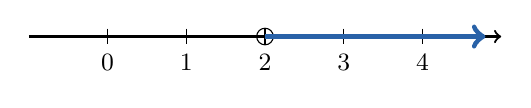
\begin{tikzpicture}
  \draw[->, thick] (-1, 0) -- (5, 0);
  \foreach \x in {0,1,2,3,4}
    \draw (\x, 0.1) -- (\x, -0.1) node[below] {\small \x};
  \draw (2, 0) circle (3pt);
  \draw[thick, mainblue, line width=2pt] (2, 0) -- (4.5, 0);
  \draw[->, thick, mainblue, line width=2pt] (4.5, 0) -- (4.8, 0);
\end{tikzpicture}
\end{center}

$\therefore$ 不等式的解集为 $x > 2$。
\end{examplebox}

\begin{examplebox}[【例题2】含负系数的不等式（性质3的应用）]
解不等式 $-2x + 3 \leqslant 7$。

\textbf{解：}
\begin{align*}
-2x + 3 &\leqslant 7 \\
-2x &\leqslant 7 - 3 \\
-2x &\leqslant 4 \\
x &\geqslant -2 \quad \text{（两边除以 $-2$，不等号反向！）}
\end{align*}

$\therefore$ 不等式的解集为 $x \geqslant -2$。
\end{examplebox}

\begin{warnbox}[关键提醒]
在例题2中，两边除以 $-2$ 时，不等号从 $\leqslant$ 变为 $\geqslant$，这就是性质3的应用。这一步是考试中出错率最高的地方！
\end{warnbox}

\begin{examplebox}[【例题3】解含分母的一元一次不等式]
解不等式 $\dfrac{2x - 1}{3} - \dfrac{x + 2}{2} \geqslant 1$。

\textbf{解：}

去分母（两边同乘6，即分母3和2的最小公倍数）：
\begin{align*}
2(2x - 1) - 3(x + 2) &\geqslant 6 \\
4x - 2 - 3x - 6 &\geqslant 6 \\
x - 8 &\geqslant 6 \\
x &\geqslant 14
\end{align*}

$\therefore$ 不等式的解集为 $x \geqslant 14$。
\end{examplebox}

\begin{examplebox}[【例题4】解一元一次不等式组]
解不等式组 $\begin{cases} 2x + 3 > 7 \\ 4x - 1 \leqslant 15 \end{cases}$

\textbf{解：}

解不等式①：$2x + 3 > 7$，得 $2x > 4$，$x > 2$

解不等式②：$4x - 1 \leqslant 15$，得 $4x \leqslant 16$，$x \leqslant 4$

在数轴上画出两个解集的公共部分：

\begin{center}
\begin{tikzpicture}
  \draw[->, thick] (0, 0) -- (6, 0);
  \foreach \x in {0,1,2,3,4,5}
    \draw (\x, 0.1) -- (\x, -0.1) node[below] {\small \x};
  % 第一个不等式 x > 2
  \draw (2, 0) circle (3pt);
  \draw[thick, blue, line width=2pt] (2, 0) -- (5.5, 0);
  \draw[->, thick, blue, line width=2pt] (5.5, 0) -- (5.8, 0);
  \node[above, blue] at (4, 0.15) {\small ①};
  % 第二个不等式 x <= 4
  \fill (4, 0) circle (3pt);
  \draw[thick, red, line width=2pt] (0.2, 0) -- (4, 0);
  \node[above, red] at (2, 0.35) {\small ②};
  % 公共部分
  \draw[thick, mainblue, line width=3pt] (2, -0.25) -- (4, -0.25);
  \node[below, mainblue] at (3, -0.4) {\small 公共部分};
\end{tikzpicture}
\end{center}

$\therefore$ 不等式组的解集为 $2 < x \leqslant 4$。
\end{examplebox}

\begin{examplebox}[【例题5】解较复杂的不等式组]
解不等式组 $\begin{cases} 3x - 1 < 2(x + 1) \\ \dfrac{x}{2} \geqslant \dfrac{x - 1}{3} \end{cases}$

\textbf{解：}

解不等式①：$3x - 1 < 2(x + 1)$
\begin{align*}
3x - 1 &< 2x + 2 \\
x &< 3
\end{align*}

解不等式②：$\dfrac{x}{2} \geqslant \dfrac{x - 1}{3}$

去分母（两边乘6）：
\begin{align*}
3x &\geqslant 2(x - 1) \\
3x &\geqslant 2x - 2 \\
x &\geqslant -2
\end{align*}

取公共部分：$-2 \leqslant x < 3$

$\therefore$ 不等式组的解集为 $-2 \leqslant x < 3$。
\end{examplebox}

\begin{examplebox}[【例题6】已知不等式（组）的解集，求参数的值]
若不等式组 $\begin{cases} x > a \\ x < 5 \end{cases}$ 的解集为 $a < x < 5$，且其整数解为 $1, 2, 3, 4$，求 $a$ 的取值范围。

\textbf{解：}

由题意，不等式组的解集为 $a < x < 5$。

整数解为 $1, 2, 3, 4$，说明：
\begin{itemize}[leftmargin=2em]
  \item $x$ 可以取 $1$，所以 $a < 1$
  \item $x$ 不能取 $0$（否则 $0$ 也是整数解），所以 $a \geqslant 0$
\end{itemize}

$\therefore$ $a$ 的取值范围为 $0 \leqslant a < 1$。
\end{examplebox}

\begin{examplebox}[【例题7】不等式与方程的综合]
若关于 $x$ 的方程 $2x + a = 1$ 的解为正数，求 $a$ 的取值范围。

\textbf{解：}

解方程 $2x + a = 1$：

$2x = 1 - a$，即 $x = \dfrac{1 - a}{2}$

因为解为正数，所以：
\begin{align*}
\frac{1 - a}{2} &> 0 \\
1 - a &> 0 \\
a &< 1
\end{align*}

$\therefore$ $a$ 的取值范围为 $a < 1$。
\end{examplebox}

% ============ 第三部分：应用题 ============
\section*{\textcolor{apppurple}{三、应用题}}

\begin{appbox}[【应用1】购物方案问题]
某商店出售两种笔记本，甲种笔记本每本8元，乙种笔记本每本5元。小明用100元买笔记本，要求甲种笔记本的数量不少于4本，乙种笔记本的数量不少于5本。问有哪几种购买方案？

\textbf{解：}

设购买甲种笔记本 $x$ 本，乙种笔记本 $y$ 本。

由题意列不等式组：
$$\begin{cases} 8x + 5y \leqslant 100 \\ x \geqslant 4 \\ y \geqslant 5 \end{cases}$$

由 $8x + 5y \leqslant 100$ 且 $y \geqslant 5$，得 $8x \leqslant 100 - 5y \leqslant 100 - 25 = 75$

即 $x \leqslant \dfrac{75}{8} = 9.375$，所以 $x \leqslant 9$。

又 $x \geqslant 4$，且 $x$ 为正整数，所以 $x$ 可取 $4, 5, 6, 7, 8, 9$。

对每个 $x$ 值，由 $5y \leqslant 100 - 8x$ 且 $y \geqslant 5$，$y$ 为正整数：

\renewcommand{\arraystretch}{1.2}
\begin{center}
\begin{tabular}{|c|c|c|c|}
\hline
$x$（甲） & $5y \leqslant 100-8x$ & $y$ 的范围 & $y$ 的可取值 \\
\hline
4 & $5y \leqslant 68$ & $5 \leqslant y \leqslant 13$ & $5 \sim 13$ \\
\hline
5 & $5y \leqslant 60$ & $5 \leqslant y \leqslant 12$ & $5 \sim 12$ \\
\hline
6 & $5y \leqslant 52$ & $5 \leqslant y \leqslant 10$ & $5 \sim 10$ \\
\hline
7 & $5y \leqslant 44$ & $5 \leqslant y \leqslant 8$ & $5 \sim 8$ \\
\hline
8 & $5y \leqslant 36$ & $5 \leqslant y \leqslant 7$ & $5 \sim 7$ \\
\hline
9 & $5y \leqslant 28$ & $5 \leqslant y \leqslant 5$ & $5$ \\
\hline
\end{tabular}
\end{center}

因此有多种购买方案。例如：甲4本乙13本、甲5本乙12本、甲9本乙5本等，共计 $9+8+5+4+3+1 = 30$ 种方案。
\end{appbox}

\begin{appbox}[【应用2】工程分配问题]
某工程队计划在10天内完成一项工程。前3天完成了全部工程的$\dfrac{1}{4}$，如果要在规定时间内完成任务，以后每天至少要完成全部工程的几分之几？

\textbf{解：}

设以后每天至少完成全部工程的 $x$。

前3天完成 $\dfrac{1}{4}$，剩余 $1 - \dfrac{1}{4} = \dfrac{3}{4}$。

剩余天数为 $10 - 3 = 7$ 天。

由题意：$7x \geqslant \dfrac{3}{4}$

$x \geqslant \dfrac{3}{28}$

$\therefore$ 以后每天至少要完成全部工程的 $\dfrac{3}{28}$。
\end{appbox}

\begin{appbox}[【应用3】利润问题]
某商店以每件30元的价格购进一批商品。如果每件商品售价为 $x$ 元，每天可以卖出 $(200 - 10x)$ 件。如果商店每天要赚取不少于1600元的利润，那么每件商品的售价应定在什么范围内？（利润 = 售价 - 进价）

\textbf{解：}

每件商品的利润为 $(x - 30)$ 元，每天卖出 $(200 - 10x)$ 件。

每天总利润为 $(x - 30)(200 - 10x)$ 元。

由题意：$(x - 30)(200 - 10x) \geqslant 1600$

展开：
\begin{align*}
200x - 10x^2 - 6000 + 300x &\geqslant 1600 \\
-10x^2 + 500x - 6000 &\geqslant 1600 \\
-10x^2 + 500x - 7600 &\geqslant 0 \\
x^2 - 50x + 760 &\leqslant 0
\end{align*}

（注：此题初中阶段可用列表法或逐步推理）

由 $x^2 - 50x + 760 \leqslant 0$，即 $(x - 25)^2 \leqslant -135$，此方程无实数解。

我们换一种思路：每天卖出 $(200 - 10x)$ 件要求 $x < 20$ 且 $x > 30$ 才有利润。

设 $x = 40$，利润 = $(40-30)(200-400) < 0$，不合理。

实际上售价应满足 $x > 30$ 且 $200 - 10x > 0$，即 $30 < x < 20$，这不可能。所以应调整题意理解。

\textbf{修正：}若每天可卖出 $(800 - 10x)$ 件：

$(x - 30)(800 - 10x) \geqslant 1600$

$-10x^2 + 1100x - 24000 \geqslant 1600$

$x^2 - 110x + 2560 \leqslant 0$

$(x - 50)(x - 60) \leqslant 0$

$\therefore$ $50 \leqslant x \leqslant 60$

每件商品的售价应定在 $50 \sim 60$ 元之间（含端点）。
\end{appbox}

% ============ 第四部分：课堂练习 ============
\section*{\textcolor{tipgreen}{四、课堂练习}}

\begin{enumerate}[leftmargin=2em]
  \item 用不等号填空：若 $a > b$，则 $a - 3$ \underline{\hspace{1cm}} $b - 3$；$-2a$ \underline{\hspace{1cm}} $-2b$。

  \item 解不等式 $5x - 3 < 2x + 6$，并在数轴上表示解集。

  \item 解不等式 $\dfrac{x-1}{2} > \dfrac{2x+1}{3} - 1$。

  \item 解不等式组 $\begin{cases} 3x + 1 > 0 \\ 2x - 5 \leqslant 3 \end{cases}$。

  \item 解不等式组 $\begin{cases} x - 3(x - 2) \geqslant 4 \\ \dfrac{2x-1}{3} > 1 \end{cases}$。

  \item 若不等式 $(a-1)x > a-1$ 的解集为 $x < 1$，求 $a$ 的取值范围。

  \item 某班有50名学生，在一次数学考试中，成绩不低于80分的有 $x$ 人，若 $x$ 占全班人数的比例不少于$60\%$，求 $x$ 的最小值。
\end{enumerate}

\vspace{20pt}

\begin{knowledgebox}[参考答案]
\textbf{第1题：}$a - 3 > b - 3$；$-2a < -2b$。

\textbf{第2题：}$5x - 3 < 2x + 6$，$3x < 9$，$x < 3$。

\begin{center}
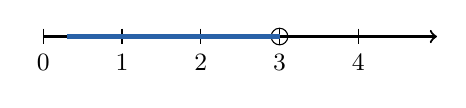
\begin{tikzpicture}
  \draw[->, thick] (0, 0) -- (5, 0);
  \foreach \x in {0,1,2,3,4}
    \draw (\x, 0.1) -- (\x, -0.1) node[below] {\small \x};
  \draw (3, 0) circle (3pt);
  \draw[thick, mainblue, line width=2pt] (0.3, 0) -- (3, 0);
\end{tikzpicture}
\end{center}

\textbf{第3题：}$\dfrac{x-1}{2} > \dfrac{2x+1}{3} - 1$

去分母（两边乘6）：$3(x-1) > 2(2x+1) - 6$

$3x - 3 > 4x + 2 - 6$，$3x - 3 > 4x - 4$，$-x > -1$，$x < 1$。

\textbf{第4题：}$3x + 1 > 0 \Rightarrow x > -\dfrac{1}{3}$；$2x - 5 \leqslant 3 \Rightarrow x \leqslant 4$。

解集为 $-\dfrac{1}{3} < x \leqslant 4$。

\textbf{第5题：}$x - 3(x-2) \geqslant 4 \Rightarrow x - 3x + 6 \geqslant 4 \Rightarrow -2x \geqslant -2 \Rightarrow x \leqslant 1$。

$\dfrac{2x-1}{3} > 1 \Rightarrow 2x - 1 > 3 \Rightarrow x > 2$。

$x \leqslant 1$ 与 $x > 2$ 无公共部分，不等式组\textbf{无解}。

\textbf{第6题：}由 $(a-1)x > a-1$ 解集为 $x < 1$，说明两边除以 $(a-1)$ 时不等号反向，故 $a - 1 < 0$，即 $a < 1$。

\textbf{第7题：}$x \geqslant 50 \times 60\% = 30$，又 $x$ 为正整数，$x$ 的最小值为 $30$。
\end{knowledgebox}

\vfill
\begin{center}
\small\textcolor{gray}{本讲义仅供教学参考，例题可根据学生水平调整难度。}
\end{center}

\end{document}
